%!TeX spellcheck=en_US
\documentclass[11pt,
               a4paper,
               bibtotoc,
               idxtotoc,
               headsepline,
               footsepline,
               footexclude,
               BCOR12mm,
               DIV13,
               openany,   % using this removes blank pages around part / chapter starts.
%               oneside    % include this if you have to print only one page per sheet of paper.
               ]
               {scrbook}

%%% SETTINGS

% no word wrapping
%\righthyphenmin=62
%\lefthyphenmin=62
% fewer hyphens
\usepackage{microtype}

% german symbols
\usepackage[utf8]{inputenc}

% strikethrough by \sout
\usepackage[normalem]{ulem}

% insert graphics
\usepackage{graphicx}
% more flexible figures e.g. graphics with captions beside them
\usepackage{floatrow}
% more flexible captions.
% Use \captionsetup{options} to configure,
% use it in an environment for local setup
\usepackage{caption}
% subfigures (see template):
\usepackage{subcaption}

% more control of enumerations and itemizations
\usepackage{enumitem}
% less space between items
\setlist[itemize]{itemsep=0cm}
\setlist[enumerate]{itemsep=0cm}
% more customizeable tables (e.g. multiple lines per cell)
\usepackage{tabularx}
% fix for vertical centering
\usepackage{ragged2e}
\renewcommand\tabularxcolumn[1]{>{\Centering}m{#1}}
% column types with multiple lines and formatting
\usepackage{array}
\newcolumntype{C}{>{\centering\arraybackslash}X}
\newcolumntype{R}{>{\raggedleft\arraybackslash}X}
\newcolumntype{L}{>{\raggedright\arraybackslash}X}
% merge multiple rows \multirow{2}{*}{bla} & \\ &
\usepackage{multirow}
% activate for tables with page breaking
%\usepackage{ltablex}
% fix for table movement and itemizations
%\keepXColumns

% fix for dynamics spaces after custom commands
\usepackage{xspace}

% tabbing: use with \tab
\usepackage{tabto}
\TabPositions{4cm}

%% fancy math
% propper matrices, underbrace text
%\usepackage{amsmath}
\usepackage{mathtools}
% special symbols e.g. squares
\usepackage{amssymb}

%% plotting
\usepackage{pgfplots}
\usepgfplotslibrary{fillbetween}

%%Settings for code
% code placement right there
\usepackage{float}
% code coloring
\usepackage{xcolor}
% code listing
\usepackage{listings}

% flexible multi column style
\usepackage{multicol}

% graphs
\usepackage{tikz}
\usetikzlibrary{shapes.geometric, arrows}
% define some elements
\tikzstyle{startstop} = [rectangle, rounded corners, minimum width=3cm, minimum height=1cm,text centered, draw=black, fill=blue!30]
\tikzstyle{arrow} = [thick,->,>=stealth]

% Some code highlighting styles you can use with lstlistings
% C++ code style similar to default eclipse
\lstdefinestyle{eclipse-cpp} {
    captionpos=b,
    language=C++,
    otherkeywords={final},
    basicstyle=\footnotesize,
    numbers=left,
    numberstyle=\small,
    showstringspaces=false,
    tabsize=2,
    frame=single,
    breaklines=true,
    keywordstyle=\bfseries\color[RGB]{127,0,85},
    identifierstyle=\color[RGB]{0,0,192},
    stringstyle=\color[RGB]{42,0,255},
    commentstyle=\color[RGB]{63,127,95},
}

% If no highlighting is intended
\lstdefinestyle{plain}{
}

% fancy algorithms (see template)
\usepackage[ruled, vlined, linesnumbered]{algorithm2e}
\DontPrintSemicolon
\SetKw{KwBy}{by}
\SetKw{KwAnd}{and}

% clickable links and clickable table of content <3
% Options: links with linebreaks
\PassOptionsToPackage{hyphens}{url}\usepackage[bookmarks=false]{hyperref}
\hypersetup{
    colorlinks,
    citecolor=black,
    filecolor=black,
    linkcolor=black,
    urlcolor=black
}
% Alterations to labels used by \autoref{}: Capitalize everyything
\def\chapterautorefname{Chapter}
\def\sectionautorefname{Section}
\def\subsectionautorefname{Subsection}
\def\algorithmautorefname{Algorithm}
\def\subfigureautorefname{Figure}
% for fully custon stuff use:
% \hyperref[custom:foo]{Custom~\ref*{custom:foo}}


\usepackage{lipsum} % for filling pages with stuff

% -------------------------------------------------------------------------------
% --------------------------------- Thesis Info ---------------------------------
% -------------------------------------------------------------------------------

% set title, authors and stuff for the cover
% docytype needs xspace because it is used within text.
\def\doctype{Bachelor's Thesis\xspace}
%\def\doctype{Master's Thesis\xspace}
%\def\doctype{Guided Research\xspace}
%\def\doctype{Interdisciplinary Project\xspace}
\def\studyProgram{Informatics}
\def\title{Implementing and benchmarking Discrete Element Method simulator using AutoPas}
% don't try translate every technical term if it would sound off
\def\titleGer{Implementierung und Benchmarking von Discrete Element Method Simulator unter Anwendung von AutoPas}
\def\author{Joon Kim}
% Prof
\def\supervisor{Univ.-Prof. Dr. Hans-Joachim Bungartz}
% PhD Candidate
\def\advisor{Manish Kumar Mishra, M.Sc.}
\def\date{Date of Submission}

\begin{document}
\frontmatter
% -------------------------------------------------------------------------------
% ---------------------------------- COVERPAGE ----------------------------------
% -------------------------------------------------------------------------------

% correct BCOR - undo at the end !!!
\def\bcorcor{0.15cm}
\addtolength{\hoffset}{\bcorcor}
\thispagestyle{empty}
\vspace{4cm}
\begin{center}
    
\includegraphics[width=4cm]{templateStuff/tumlogo.pdf}\\[5mm]
    \huge SCHOOL OF COMPUTATION, INFORMATION AND TECHNOLOGY\\[5mm]
    \large DER TECHNISCHEN UNIVERSITÄT MÜNCHEN\\[24mm]

    {\Large \doctype in \studyProgram}\\[20mm]
    {\huge\bf \title\par}
    \vspace{15mm}
    {\LARGE  \author}
\end{center}

\cleardoubleemptypage

% -------------------------------------------------------------------------------
% ---------------------------------- TITLEPAGE ----------------------------------
% -------------------------------------------------------------------------------

\def\bcorcor{0.15cm}
\addtolength{\hoffset}{\bcorcor}
\thispagestyle{empty}
\vspace{10mm}
\begin{center}
    
\includegraphics[width=4cm]{templateStuff/tumlogo.pdf}\\[5mm]
	\huge SCHOOL OF COMPUTATION, INFORMATION AND TECHNOLOGY\\[5mm]
	\large DER TECHNISCHEN UNIVERSITÄT MÜNCHEN\\[24mm]
	{\Large \doctype in \studyProgram}\\[20mm]
	{\LARGE\bf \title}\\[10mm]
	{\LARGE\bf \titleGer}\\[10mm]
	\begin{tabular}{ll}
		\Large Author:      	& \Large \author \\[2mm]
		\Large Supervisor:  	& \Large \supervisor\\[2mm]
		\Large Advisor:			& \Large \advisor\\[2mm]
		\Large Date:       		& \Large \date
	\end{tabular}
\end{center}

% undo BCOR correction
\addtolength{\hoffset}{\bcorcor}
\newpage

% -------------------------------------------------------------------------------
% ---------------------------------- DISCLAIMER ---------------------------------
% -------------------------------------------------------------------------------

\cleardoubleemptypage

\thispagestyle{empty}
\vspace*{0.7\textheight}
\noindent
I confirm that this \MakeLowercase{\doctype} is my own work and I have documented all sources and material used.\\

\vspace{15mm}
\noindent
Munich, \date \hspace{5cm} \author
\cleardoubleemptypage

% -------------------------------------------------------------------------------
% ------------------------------- ACKNOWLEDGEMENTS ------------------------------
% -------------------------------------------------------------------------------

\phantomsection
\addcontentsline{toc}{chapter}{Acknowledgements}
\vspace*{2cm}
\begin{center}
    {\Large \bf Acknowledgements}
\end{center}
\vspace{1cm}

\lipsum[1]

\cleardoublepage

% -------------------------------------------------------------------------------
% ---------------------------------- ABSTRACT -----------------------------------
% -------------------------------------------------------------------------------

\phantomsection
\addcontentsline{toc}{chapter}{Abstract}
\vspace*{2cm}
\begin{center}
    {\Large \bf Abstract}
\end{center}
\vspace{1cm}

\lipsum[2]

\cleardoublepage

\phantomsection
\addcontentsline{toc}{chapter}{Zusammenfassung}
\vspace*{2cm}
\begin{center}
    {\Large \bf Zusammenfassung}
\end{center}
\vspace{1cm}

\lipsum[2]

\cleardoublepage

% -------------------------------------------------------------------------------
% ------------------------------ TABLE OF CONTENTS ------------------------------
% -------------------------------------------------------------------------------

\tableofcontents
\thispagestyle{empty}
\cleardoubleemptypage

% -------------------------------------------------------------------------------
% --------------------------------- MAIN MATTER ---------------------------------
% -------------------------------------------------------------------------------

\mainmatter
\part{Introduction}
\chapter{Introduction}
\label{sec:introduction}
The Discrete Element Method (DEM) usually attempts to gain microscopic understanding by modeling macroscopic specific behaviors. By assuming contact laws from physics and the rigidity of granular bodies, it simulates the interactions of samples. 

DEM has been widely used in the field of granular science due to its many advantages  when compared to a continuous modeling of granular materials: It is simple physics and provides insights into local quantities of individual granular bodies that could be out of reach in case of continuous modeling.

This thesis focuses on the application of AutoPas, a high-performance, auto-tuned particle simulation library for N-body systems, building a DEM simulator and benchmarking different experimental results.

\part{Background}
\chapter{Discrete spherical particle model}
\label{sec:discrete_spherical_particle_model}

The body shape of granular materials that are subjects of DEM simulations could be various. For example, sand has its specific cristal shape, which might differ from other grains such as corn or salt. 
To simplify the modeling and implementation, we assume the spherical shape of the granular units, in which the mass is uniformly distributed over its volumne.
Moreover, soft and elastic unit can undergo deformations under stress. Again, for simplicity reasons, we ignore such elastic/plastic deformations and assume an unchangable spherical shape of particles.

Ignoring the complicated stress distribution, the interaction forces in DEM only rely on the overlap between colliding two particles. As a consequence, the produced results below are of the same quality as the simplified modeling decision made here. 

    \begin{figure}[H] % [H] for HERE
	\centering
	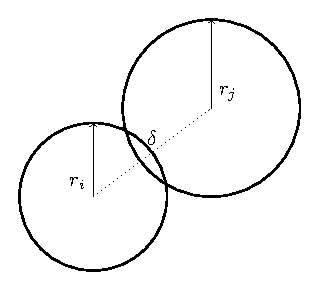
\includegraphics[width=.3\columnwidth]{figures/discrete_spherical_particle_model.pdf}
	\caption[Example Figure]{Two spherical particles in contact with overlap $\delta$ \\
		\tiny{Source: \cite{gratl17task}}}
	\label{fig:discrete_spherical_particle_model} % labels always have to be placed after the caption
\end{figure}

\chapter{Equations of Motion}
The dynamics of granular particles can be expressed with Newton's equations, which can be reduced to a system of ordinary differential equations of translational and rotational  motion:
\begin{equation}
	m_i \frac{\mathrm{d}^2}{\mathrm{d}t^2} r_i = f_{contact} + f_{global}, \quad \text{and} \quad
	I_i \frac{\mathrm{d}^2}{\mathrm{d}t^2} \varphi_i = q_{contact} + q_{global}
\end{equation}
with the mass $m_i$  of particle $i$ and its position $r_i$. The $f_{contact}$ can be obtained by the sum of all contact forces directed to particle $i$ as we assume existing interaction force when contact between two particles is present:
\begin{equation}
f_{contact} = \sum_{j \in C_{i}, i \neq j}^{} f_{ij},
\end{equation}
with $C_i$ being the set of all particles in contact with $i$. In case of present walls or reflective boundary conditions (BC), the forces ensuring such BC should be added into $f_{contact}$.
The global force $f_{global}$ expresses a force that applies to all particles in a system e.g. gravity or background friction.

Similar applies to the equations for rotational motion: the moment of inertia $I_i$ of particle $i$, which can be reduced to the closed form solution $I_i = \frac{2}{5} m_i  r_i^2$ due to the aforementioned spherical body assumption, and its angular position $\varphi_i$. The $q_{contact}$ expresses the sum of all torques rising from its contacts with other particles:
\begin{equation}
	q_{contact} = \sum_{j \in C_{i}, i \neq j}^{} q_{ij},
\end{equation}
Such torques  can rise from a tangential force, rolling and torsion as will be discussed later.
Similar to $f_{global}$, the global torque $q_{global}$, e.g. background friction, is subjected to all particles in the system.

For a $D$-dimensional simulation, each particle has $D$ translational degrees of freedom (DF), due to the $D$-dimensional coordinate axes, and $\frac{D(D-1)}{2}$ rotational DF, due to the number of possible rotational planes e.g. $xy$, $yz$, and $xz$ planes. This results in  $D + D(D-1)/2$ ODEs for each particle, that are coupled due to the tangential force, which also affects the tangential torque.

For approximating the solutions of these ODEs, numerical integrators can be applied, which will be presented next.


\chapter{Time Discretization}
\chapter{Contact Force Laws}

\part{Implementation}

\part{Benchmarking}

\part{Fake Introduction and Background}
\chapter{Fake Introduction}
\label{sec:intro}       % labels can be put almost anywhere and can be referencef from anywhere.
Write some useful intro. Here are tips along the way:

\section{Tips}
\subsection{How to Describe}
% optional: set the spacing between columns
\setlength{\columnsep}{30 pt}
When listing several points you have three basic options:
\begin{multicols}{3}
    \begin{itemize}
        \item itemize
        \item enumerate
        \item description
    \end{itemize}

    \vfill\null
    \columnbreak

    \begin{enumerate}
        \item itemize
        \item enumerate
        \item description
    \end{enumerate}

    \vfill\null
    \columnbreak

    \begin{description}
        \item[itemize] short, unordered
        \item[enumerate] short ordered
        \item[description] listing of descriptions. Also nice for longer ones.
    \end{description}

\end{multicols}


\subsection{How to Quote}

\begin{quote}
    "This is a quote!"
\end{quote}

\begin{itemize}
    \item Citations to a source can be made like this \verb|\cite{gratl17task}| =~\cite{gratl17task}
    \subitem Always join text and the citation with a non-breaking space: \verb|text~\cite{foo}|.
    \item Referencing Sections, Figures, Tables, Formulas: \verb|\autoref{sec:intro}| = \autoref{sec:intro}.
    \item Footnotes for url or further notes: \verb|\footnote{\url{https://www.top500.org}}| = \footnote{\url{https://www.top500.org}}
\end{itemize}

\subsection{How to Math}

Use the align environment for equations especially if you want to align them somehow.

\begin{align}
1 + 1 &\ne 3\\
\left(\dfrac{10}{1}\right) - 9 &= 1
\end{align}

% if you need a pagebreak because figure placement is broken:
\clearpage

\section{Environments}

\subsection{How to Figure}

Anything can also be put in multiple columns.

\begin{multicols}{2} % defines an environment with two columns
    \begin{figure}[H] % [H] for HERE
        \centering
        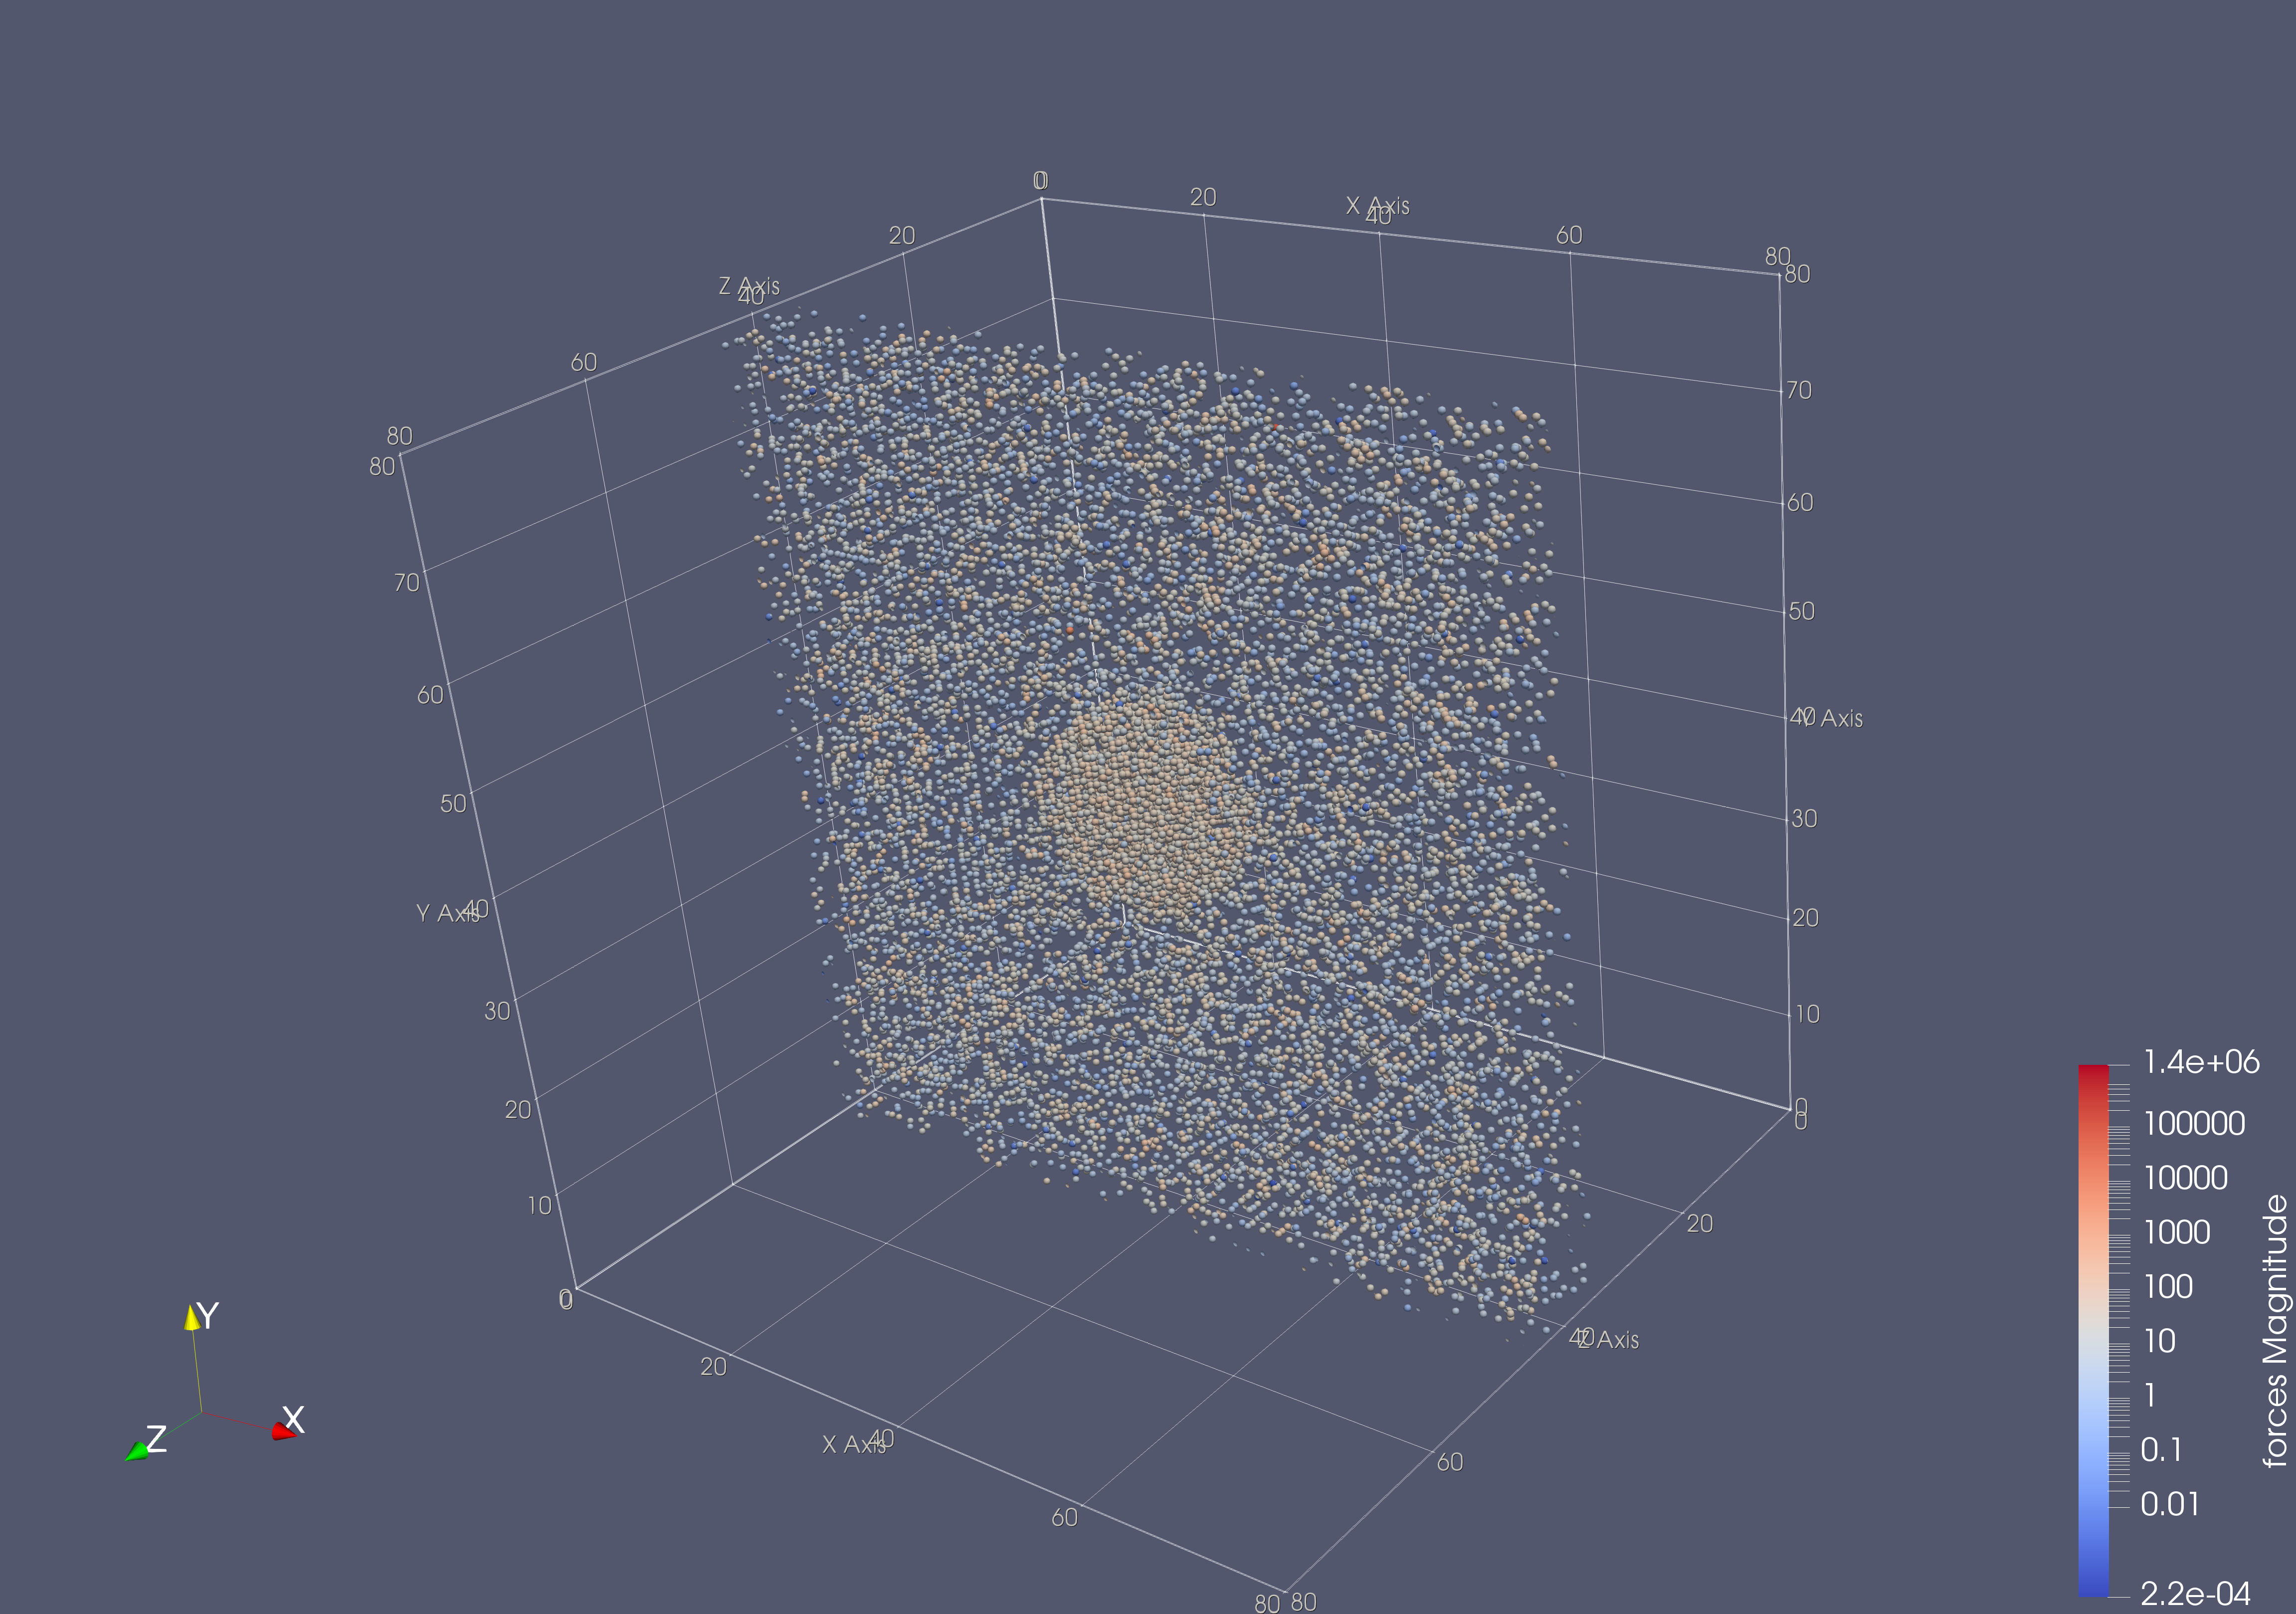
\includegraphics[width=.9\columnwidth]{figures/scenario_clip_rot.png}
        \caption[Example Figure]{Some Caption. Always also include a source if it wasn't created by you!\\
            \tiny{Source: \cite{gratl17task}}}
        \label{fig:exampleLabel1} % labels always have to be placed after the caption
    \end{figure}

    \columnbreak    % start next column

    \begin{figure}[H]
        \centering
        \begin{tikzpicture}
            \node[anchor=south west,inner sep=0] (image) at (0,0) {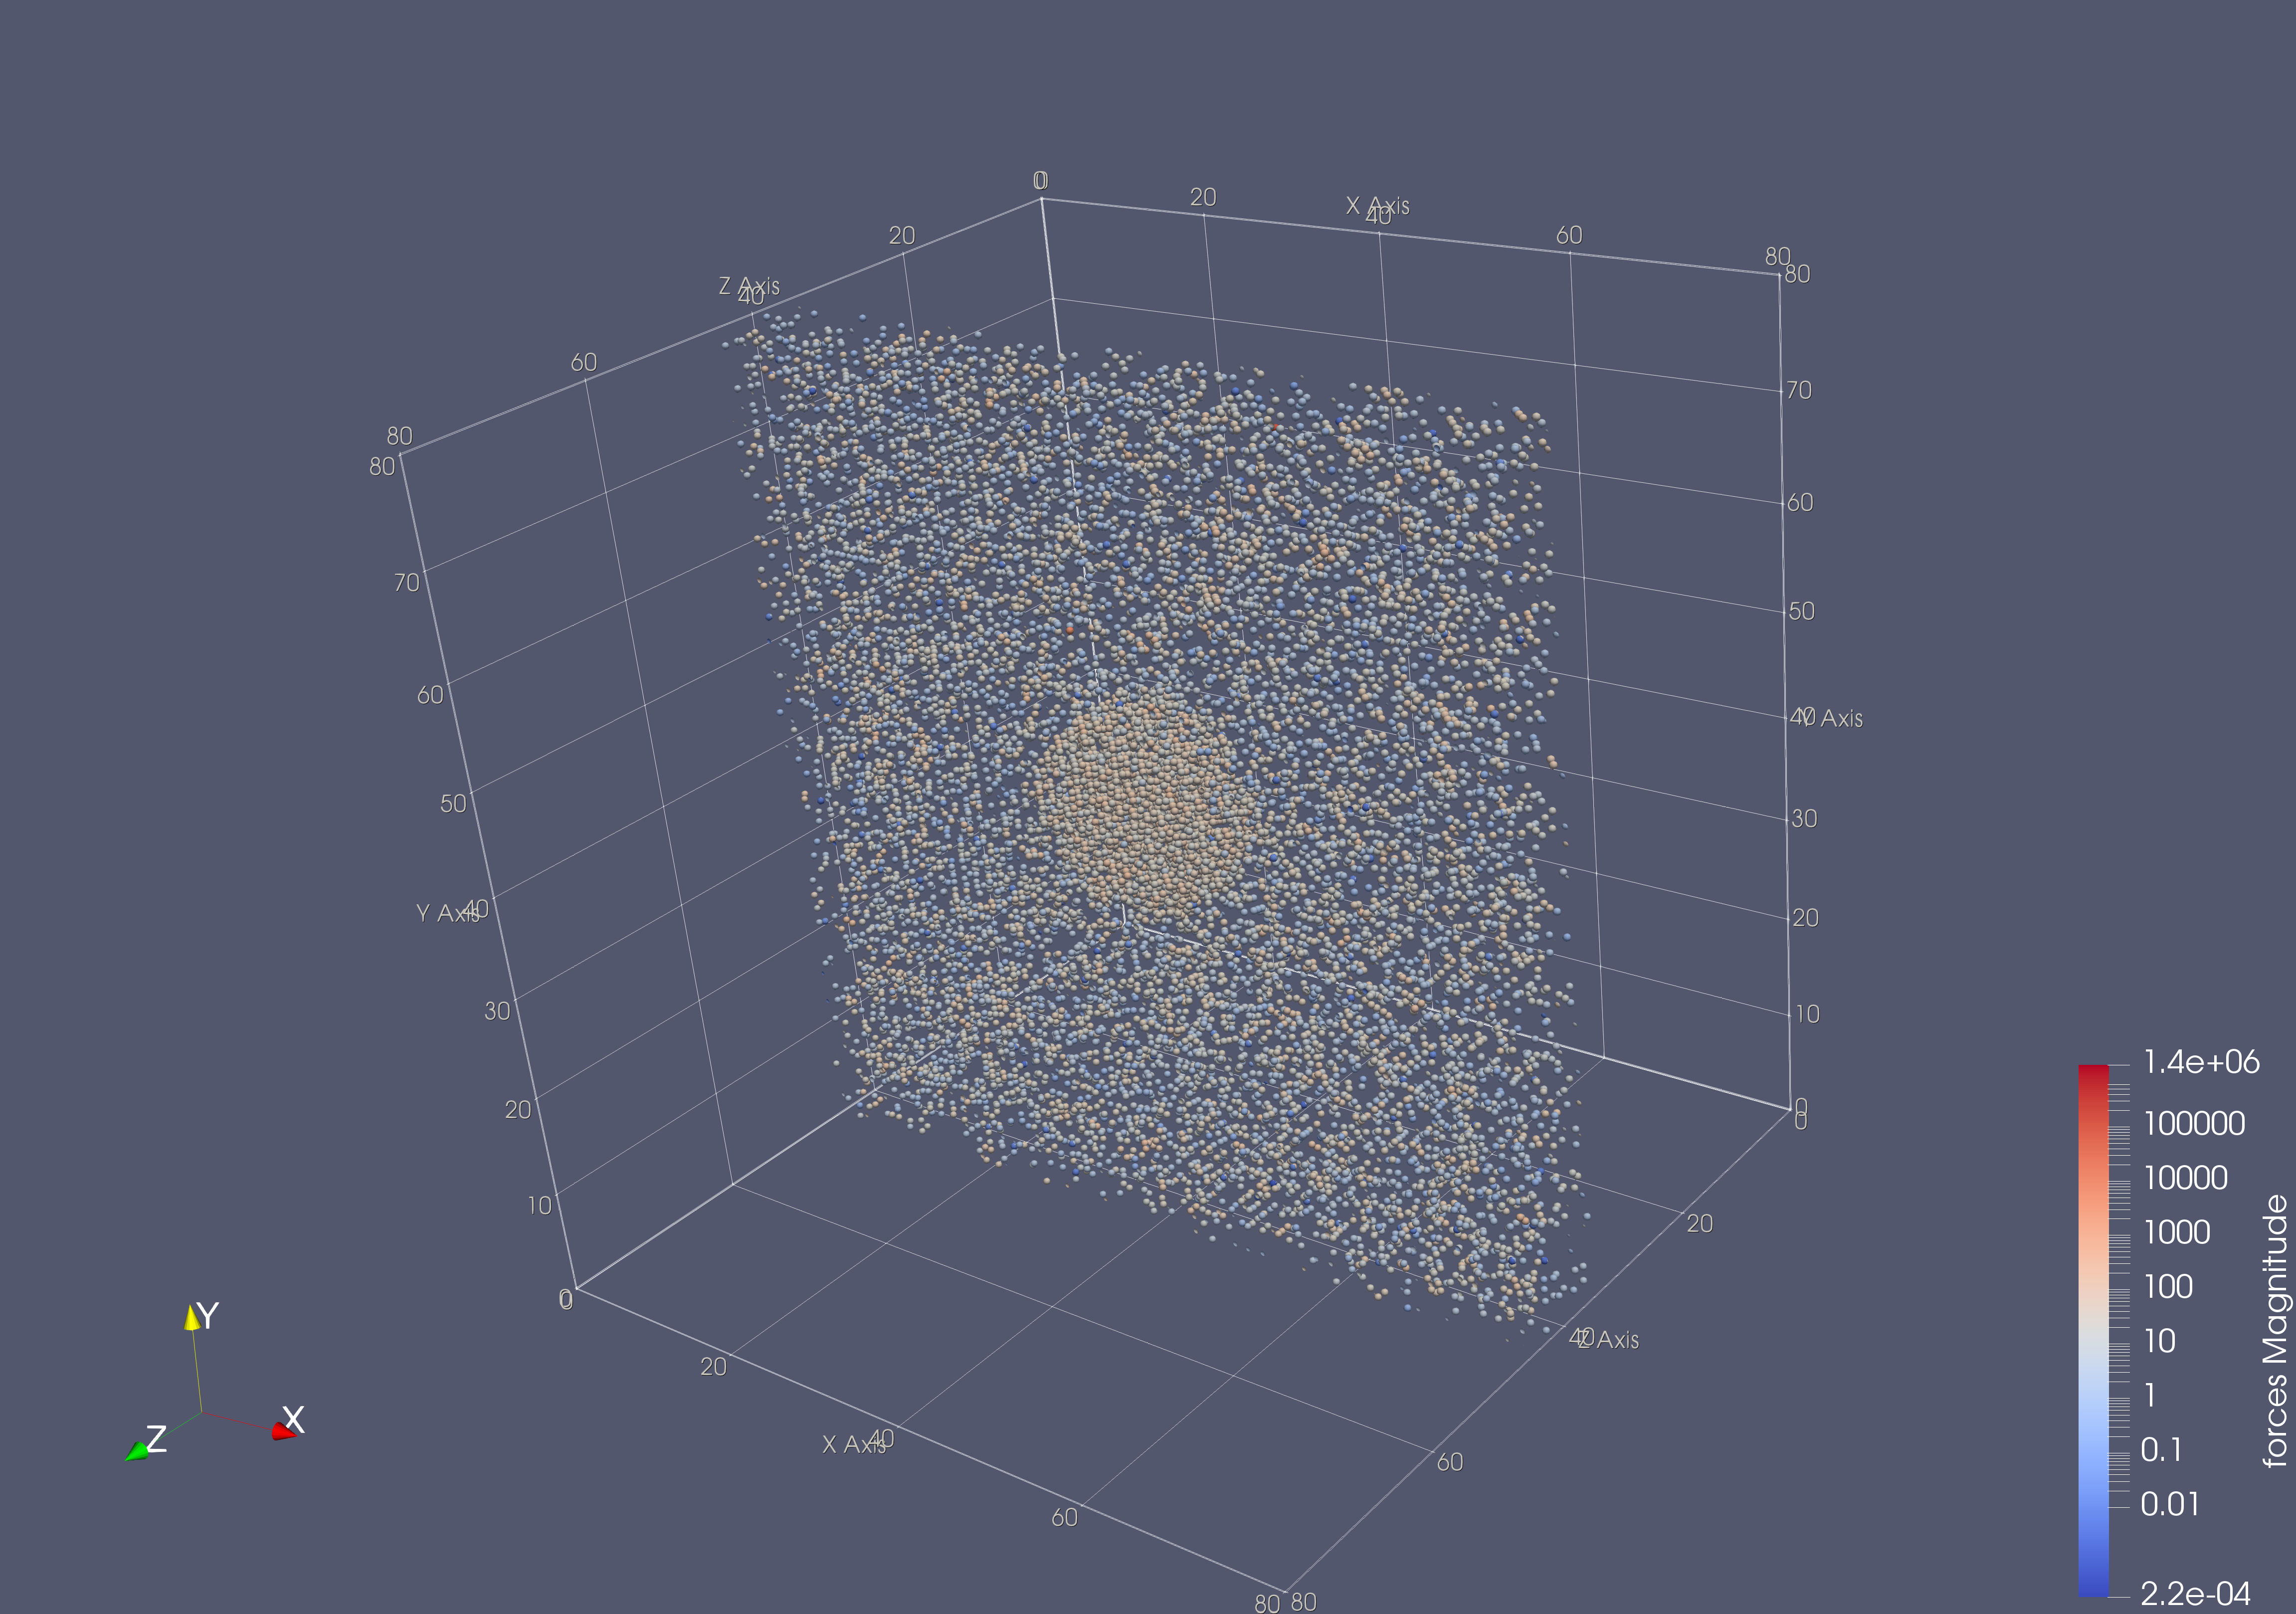
\includegraphics[width=.9\columnwidth]{figures/scenario_clip_rot.png}};
            \begin{scope}[x={(image.south east)},y={(image.north west)}]
            \draw[red, thin,rounded corners] (.42,.42) rectangle (.58,.6);
            \end{scope}
        \end{tikzpicture}
        \caption[Figure with tikz]{Figures can be drawn on or completely generated with tikz.}
        \label{fig:exampleLabel2}
    \end{figure}
\end{multicols}

\paragraph{Subfigures}
If grouping of several pictures seems reasonable, think about using subfigures. This often comes in handy with plots.

\begin{figure}[H]
    \centering
    \begin{subfigure}[b]{0.33\textwidth}
        \includegraphics[width=\textwidth]{example-image-a}
        \caption{example-image-a}
        \label{fig:example-image-a}
    \end{subfigure}
    \begin{subfigure}[b]{0.33\textwidth}
        \includegraphics[width=\textwidth]{example-image-b}
        \caption{example-image-b}
        \label{fig:example-image-b}
    \end{subfigure}
    \begin{subfigure}[b]{0.33\textwidth}
        \includegraphics[width=\textwidth]{example-image-c}
        \caption{example-image-c}
        \label{fig:example-image-c}
    \end{subfigure}
    \caption{One caption to describe them all.}
\end{figure}

\subsection{How to Algorithm}

\begin{figure}
\begin{algorithm}[H]

% Define custom keywords
\SetKwFunction{KwNot}{not}
% Define custom Functions
\SetKwFunction{Fissorted}{is\_sorted}
\SetKwFunction{Fbogosort}{bogosort}
\SetKwFunction{Fshuffle}{shuffle}
\SetKwProg{Fn}{Function}{:}{}
\KwIn{\tabto{2cm}data array}
\KwOut{\tabto{2cm} data sorted}
\BlankLine

\tcp{Checks if array is sorted}
\Fn{\Fissorted{data}}{
    \For{i $\leftarrow$ 0 \KwTo data.size() - 1}{
    \label{algo:for}            % labels can also be put in the algorithm
        \If{data[i] $>$ data[i+1]}{
            \Return false
        }
    }
    \Return true
}

\tcp{actual algorithm}
\Fn{\Fbogosort{data}}{
    \While{\KwNot \Fissorted{data}}{
        random.\Fshuffle{data}
    }
}

\caption[Bogosort]{Bogosort}
\label{algo:example}
\end{algorithm}
\caption{some description what is happening}
\end{figure}

\clearpage

\subsection{How to Code}
\begin{lstlisting}[style=eclipse-cpp, caption=General form of a typical runner() function., label=code:runner]
void runner(int type, void *data){
    switch(type)
        case taskType1:
            // do stuff using data
        case taskType2:
            // do other stuff using data
}
\end{lstlisting}

\subsection{How to Table}
\begin{table}[H]
    \begin{tabularx}{\columnwidth}{L | C | R}
        \hline
        \hline
        bla left & bla centered\newline over two lines &  bla right\\
        \hline
        bla left & bla centered & \multirow[c]{2}{\hsize}{cell spanning two rows} \\
        \cline{1-2}
        \multicolumn{2}{c|}{cell spanning two columns} & \\
    \end{tabularx}
    \caption[Some Table]{Fancy table that can contain line breaks and extended cells.}
    \label{tab:example}
\end{table}

\appendix
\part{Appendix}
\chapter{Some more stuff}

For everything that does not really belong in the thesis but is good to mention.

\listoffigures

\listoftables

\bibliographystyle{alpha}
\bibliography{literature}

\end{document}
